
\section{結果と考察}
\subsection{各用途に合わせた原子配列の表示結果}
\subsubsection{構造緩和による原子移動の表示}
構造緩和は,最安定の原子配列を検証するために,動かす前後のエネルギーを比較して原子を動作させる手法である.
図11は,この操作によって移動した原子配列の三面図である.

\begin{figure}[htbp]\begin{center}
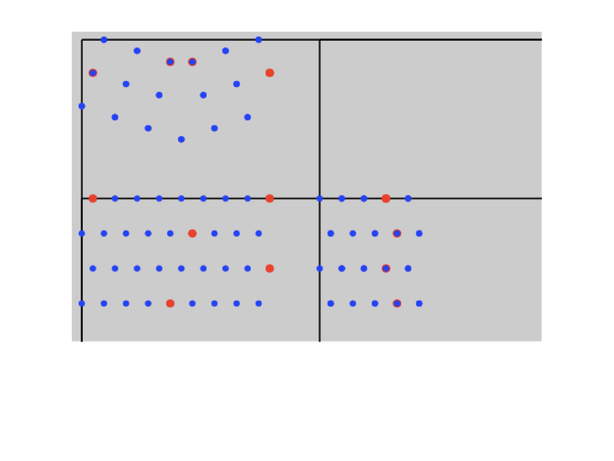
\includegraphics[width=6cm,bb=0 0 442 432]{../figs/./boundary_narita.010.jpg}
\caption{}
\label{default}\end{center}\end{figure}
図中の緑線は,構造緩和をおこなう前後で各原子が移動した経路である.
この表示結果により,第一原理計算ソフトVASPによる系全体のエネルギーを計算する際の構造緩和に過ちが生じていないかを
容易に判断できるようになった.

\subsubsection{削除された原子の識別表示.}
原子の削除操作は,岩佐の研究で最安定の原子配列の構造を探索するために取り入れた手法であり,削除された原子の位置を視覚的に把握しやすくするためにおこなった
図10は,削除されたか否かで色分けした原子配置の三面図である.

\begin{figure}[htbp]\begin{center}
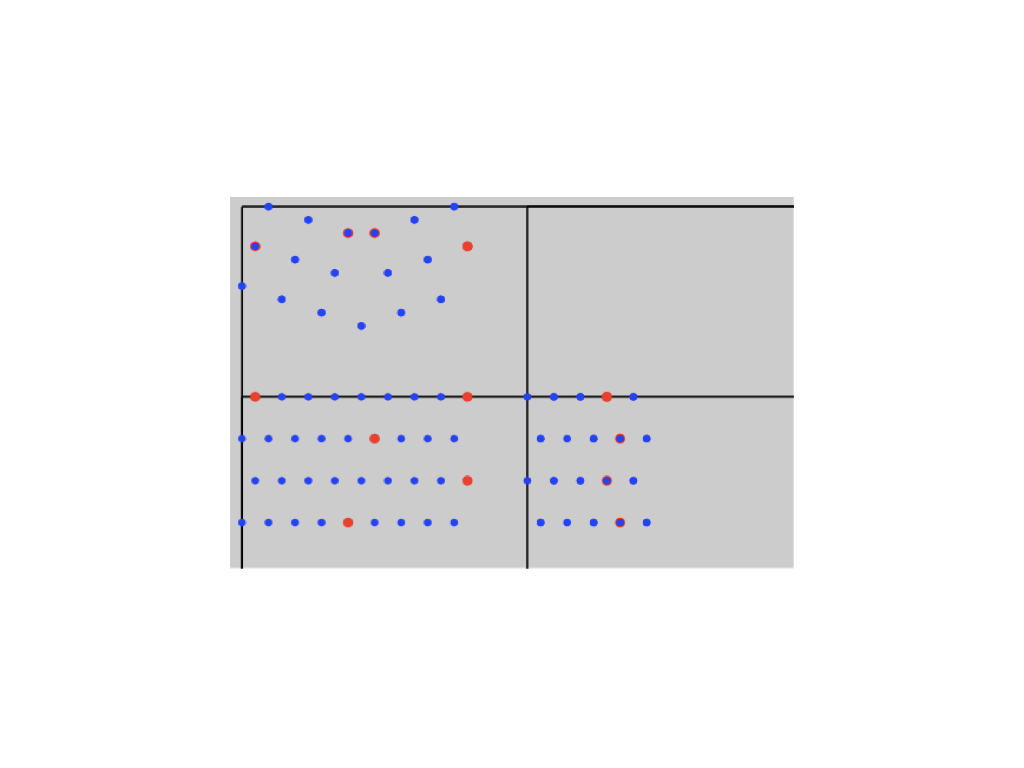
\includegraphics[width=6cm,bb=0 0 442 432]{../figs/./boundary_narita.011.jpg}
\caption{}
\label{default}\end{center}\end{figure}
図中の赤い球が削除された原子に相当する.
三面図で描画したことにより,削除された原子数,並びに各々の配置をすぐに把握することができた.

\subsubsection{指定した層の白抜き表示}
POSCAR\_2223は4層の原子配列で構成されているため,原子配列を上から見た図,すなわち平面図では,原子同士が重なって配置してしまう.
したがって,指定した層の原子が上から見てどこに位置するのかを視覚的に確認できるために原子の白抜き処理をおこなった.
z軸の3層目を白抜きしたものは,図12のように表示された.

\begin{figure}[htbp]\begin{center}
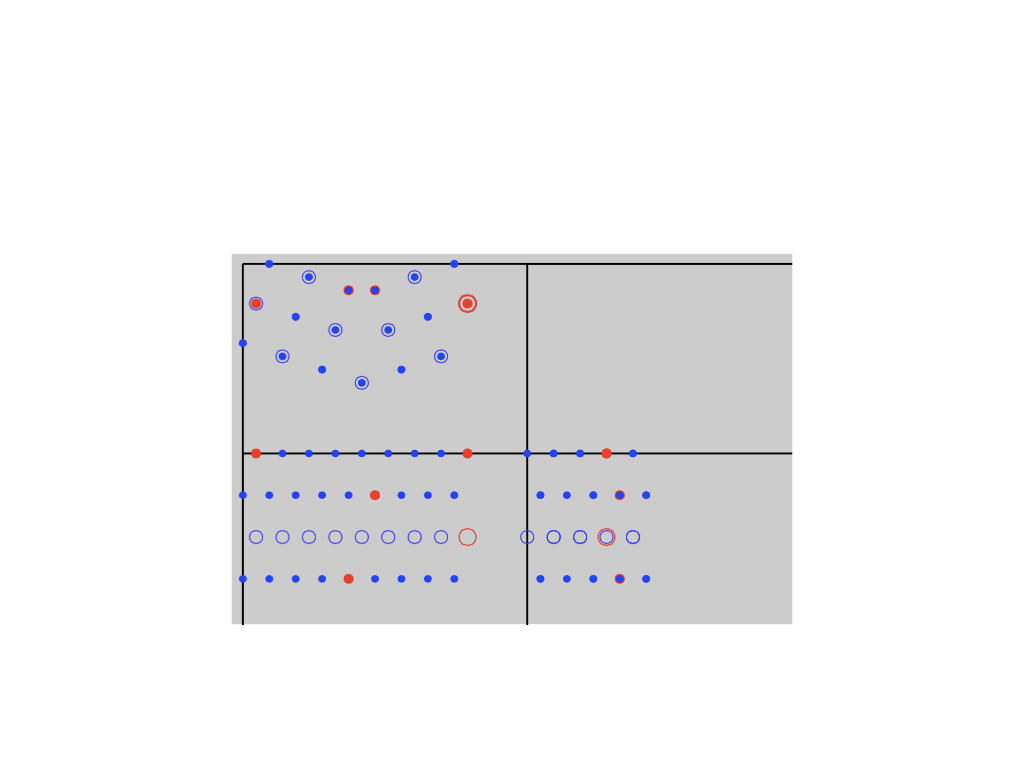
\includegraphics[width=6cm,bb=0 0 442 432]{../figs/./boundary_narita.012.jpg}
\caption{}
\label{default}\end{center}\end{figure}
\subsection{原子構造の改善点}
viewerによって三方向の視点で原子配列を表示した結果,構造緩和をおこなうためのPOSCARファイルに原子が一つ不足していることが分かった.
不足していた原子の位置は,図13の赤枠部分である.

\begin{figure}[htbp]\begin{center}
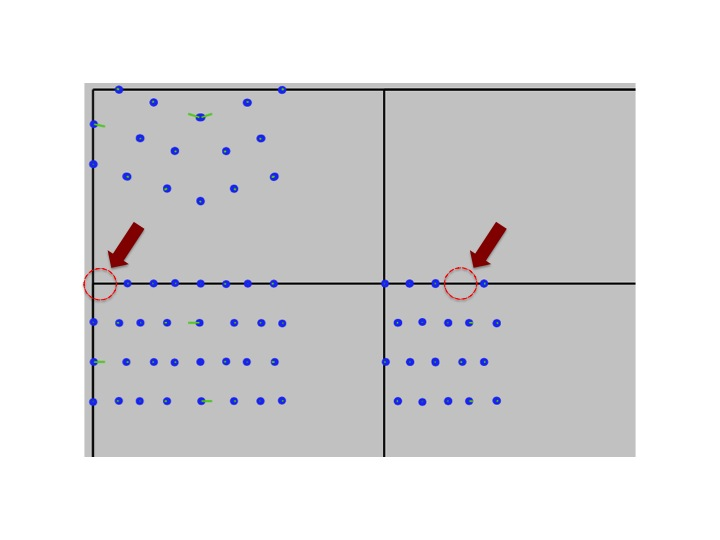
\includegraphics[width=6cm,bb=0 0 442 432]{../figs/./boundary_narita.013.jpg}
\caption{}
\label{default}\end{center}\end{figure}
これまでの原子配列は,結晶構造描画ソフト"VESTA"による三次元表示であったため,原子の細かい位置が確認できず,原子が不足していることを認識できなかった.
この結果により,構造緩和をおこなう際に使用したPOSCARファイルに過ちがあったことを発見できた.

\subsection{考察と今後の課題}
